% -*- coding: utf-8 -*-

% NOTER TIL DETTE AFSNIT:
% - API, split/sort/etc, NVIDIA, CPU
% - scan, map, split, sort
% - graf over (antal, tid)
% - Hvor meget tid bruger vi på hukommelseskopiering?

% Benchmarks af vores og andres:
%   host single thread vs vores device multi thread
%   nvidias scan vs vores scan
%   host single thread vs vores device multi thread sortering
\section{Tidsforbrug}
\label{Benchmarks}

Vi har målt tidsforbruget for hver af de primitiver vi har implementeret
og de funktioner vi har bygget ovenpå, ved at køre dem på en række vektorer af 
kvadratisk voksende størrelser, og tage gennemsnittet af ti kørsler for hver 
størrelse. Tallene kan ses i bilag \ref{benchmark-data}.

De funktioner der er bygget ovenpå scan, har vi målt både med vores egen implementation
af scan, og med NVIDIAs implementation, som vi har modificeret til at bruge \verb|int|
istedet for \verb|float|. Den modificerede kode kan ses i bilag 
\ref{code-nvidia-scan}, \ref{code-nvidia-kernel} og \ref{code-nvidia-large-kernel}.

Vi har hverken medtaget den indledende allokering af hukommelse eller den efterfølgende 
frigørelse i vores målinger. Ind- og uddata ligger på grafikkortet.
På den måde kan vi få de mest sigende tal for mindre vektorer.

Vi har desuden implementeret CPU-versioner af funktionerne og målt tidsforbruget for
dem for at have en reference. Funktionerne ganske simple, og CPU-versionen af radix-sort
arbejder på samme måde som GPGPU-versionen med et bit ad gangen.
Koden for disse implementationer kan ses i bilag 
\ref{code-cpu-map}, \ref{code-cpu-scan}, \ref{code-cpu-split} og \ref{code-cpu-radix}.

Koden for målingerne kan findes i bilag \ref{code-test}. 

Vi har målt op til $2^{23}$ elementer. Vores scan understøtter ikke flere, og NVIDIAs
scan understøtter også kun op til $2^{24}$.

Vi har målt på et grafikkort af typen NVIDIA GeForce GTX 260, 
og et værtssystem af typen Intel Core2 Quad CPU @ 2,66 GHz.

Alle diagrammerne i dette afsnit viser hvor lang tid (i millisekunder ud af y-aksen)
det tager at køre en algoritme på vektorer af forskellige størrelser 
(antal elementer ud af x-aksen). Begge akser er logaritmiske.

\subsection{Elementvise primitiver}

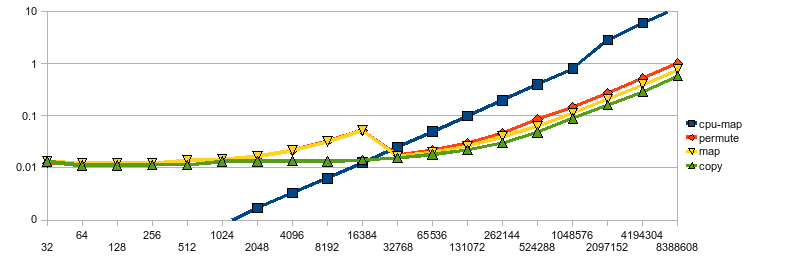
\includegraphics[width=1.0\textwidth]{bench-map.png}

Ved omkring $2^{15}$ elementer bliver vores GPGPU-implementation af map hurtigere end en
simpel CPU-version, og er mod slutningen ca. 15 gange hurtigere. 
De andre elementvise primitiver ligger tæt op af map i tidsforbrug.

\subsection{Scan}

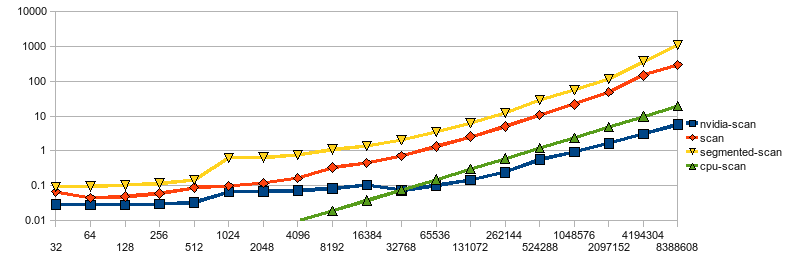
\includegraphics[width=1.0\textwidth]{bench-scan.png}

Ved omkring $2^{15}$ elementer bliver NVIDIAs GPGPU-baserede scan-implementation hurtigere 
end en simpel implementation på CPU'en.

Vores implementation af scan bliver derimod ikke hurtigere for de størrelser
vi har målt, og hvis kurven ekstrapoleres nærmer de sig heller ikke CPU-versionen. Hen mod 
slutningen af kurven er den ca. 60 gange langsommere end NVIDIAs implementation. 
Vores segmented scan er til sidst ca. fire gange langsommere end vores scan.

For store vektorer er NVIDIAs scan ca. tre gange hurtigere end CPU-versionen.

Springet på kurven for mellem 512 elementer og 1024 elementer er sandsynligvis et resultat 
af at gå fra en enkelt til to blokke, idet der som beskrevet i afsnit \ref{CUDA} kun 
kan være 512 tråde i en blok.

\subsection{Split}

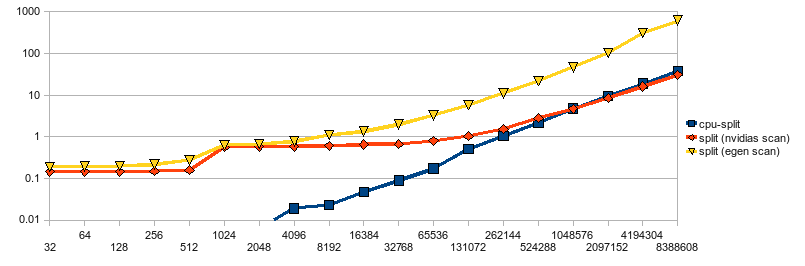
\includegraphics[width=1.0\textwidth]{bench-split.png}

Springet fra scan skinner igennem på denne kurve, da vi bruger scan i implementationen.

Det relativt mindre forhold mellem implementationen med vores scan og NVIDIAs scan kommer
af at vi udover scan også bruger de relativt hurtige elementvise primitiver.

GPGPU-versionen af split bliver aldrig markant hurtigere end den simple CPU-version,
heller ikke selvom vi anvender NVIDIAs scan.

I starten af kurven er omkostningen ved NVIDIAs scan høj, men den bliver relativt mindre
for større vektorer. NVIDIAs scan kun er tre gange hurtigere end en simpel summering på 
CPU'en (cpu-scan), og da hver iteration af cpu-radix ikke er meget mere kompleks end en
summering giver det mening at den er stort set lige så hurtig.

\subsection{Radix sort}

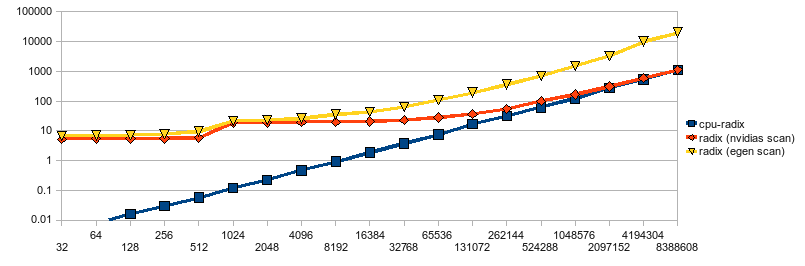
\includegraphics[width=1.0\textwidth]{bench-radix.png}

Da størstedelen af arbejdet i vores radix sort foregår i split-funktionen,
ligner kurven for de to funktioner ikke overraskende hinanden. 

